% file's preambule

\usepackage[T2A]{fontenc}
\usepackage[utf8]{inputenc}
\usepackage[english,russian]{babel} 
\usepackage{amsmath} 
\usepackage{
amssymb,textcomp, esvect,esint}
\usepackage[margin=1in]{geometry}
\usepackage{titling} 
\usepackage{amsfonts}
\usepackage{amsthm}
\usepackage{graphicx}
\usepackage{indentfirst} 
\usepackage{xcolor} 
\usepackage{enumitem}
\usepackage[unicode, pdftex]{hyperref}
\usepackage{booktabs}
\usepackage{caption}
\usepackage{listings}
\usepackage{multirow}
\usepackage{pifont}
\usepackage{cancel}
\usepackage{ulem}

\usepackage{import}
\usepackage{xifthen}
\usepackage{pdfpages}
\usepackage{transparent}
\usepackage{tikz}


% \newcommand{\incfig}[1]{%
%     \def\svgwidth{\columnwidth}
%     \import{./img/}{#1.pdf_tex}
% }

%%%%%%%%%%%%%%%%%%%%%%%%%%%%%%%%%%%%%%%%%%%%%%%%%%%%%%%%%%%%%%%%%%%%%%%%
\newcommand{\Ker}{\mathop{\mathrm{Ker}}\nolimits}
\renewcommand{\Im}{\mathop{\mathrm{Im}}\nolimits}
\newcommand{\diag}{\mathop{\mathrm{diag}}\nolimits}
\renewcommand{\Re}{\mathop{\mathrm{Re}}\nolimits}
\newcommand{\Spec}{\mathop{\mathrm{Spec}}\nolimits}
\renewcommand{\d}{\, d}
\newcommand{\A}{\mathcal A}
\newcommand{\N}{\mathcal N}
\renewcommand{\leq}{\leqslant}
\renewcommand{\geq}{\geqslant}
\renewcommand{\L}{\mathcal{L}}
\newcommand{\vc}[1]{\mbox{\boldmath $#1$}}
\newcommand{\T}{^{\text{T}}}
\newcommand{\sign}{\text{sign}}
\newcommand{\red}[1]{\textcolor{red}{#1}}
\newcommand{\const}{\text{const}}
\newcommand{\lr}[1]{\left(#1\right)}
\newcommand{\oo}{\mathop{\mathrm{o}}\nolimits}
\newcommand{\OO}{\mathop{\mathrm{O}}\nolimits}
\newcommand{\xmark}{\ding{55}}
\newcommand*\socrat{
\includegraphics{socrat.pdf}}
\newcommand*\koz{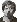
\includegraphics{koz.pdf}}
\newcommand{\F}{\mathbb{F}}  
\newcommand{\Sp}[2]{(\vc{#1}, \vc{#2})}
\newcommand{\norm}[1]{\|\vc{#1}\|}
\newcommand{\ten}{\mathbb{T}}
\newcommand{\numt}{T_{i_1, \dots, i_p}^{j_1, \dots, j_p}}
\newcommand{\vR}[1]{V_{#1}(\mathbb{R})}
\newcommand{\tr}{\text{tr}}
\newcommand{\rg}{\mathop{\mathrm{rg}}\nolimits}
%%%%%%%%%%%%%%%%%%%%%%%%%%%%%%%%%%%%%%%%%%%%%%%%%%%%%%%%%%%%%%%%%%%%%%%%

\makeatletter %%%%%%%%%%%%%%% КРУЖОЧЕК %%%%%%%%%%%%%%%
\newcommand*{\encircled}[1]{\relax\ifmmode\mathpalette\@encircled@math{#1}\else\@encircled{#1}\fi}
\newcommand*{\@encircled@math}[2]{\@encircled{$\m@th#1#2$}}
\newcommand*{\@encircled}[1]{%
  \tikz[baseline,anchor=base]{\node[draw,circle,outer sep=0pt,inner sep=.2ex] {#1};}}
\makeatother

\usepackage{arydshln} %%%%%%%%%%%%%%% ЛИНИИ В МАТРИЧКЕ %%%%%%%%%%%%%%%
\makeatletter
  \renewcommand*\env@matrix[1][*\c@MaxMatrixCols c]{%
    \hskip -\arraycolsep
    \let\@ifnextchar\new@ifnextchar
  \array{#1}}
\makeatother


\newtheorem{to_thr}{Thr}[section]
\newtheorem{to_suj}{Suj}[section]
\newtheorem{to_lem}{Lem}[section]
\newtheorem{to_com}{Com}[section]
\newtheorem{to_con}{Con}[section]
\theoremstyle{definition}
\newtheorem{to_def}{Def}[section]

\definecolor{darkblue}{HTML}{000099}
\definecolor{linkcolor}{HTML}{0000CC}
\definecolor{urlcolor}{HTML}{006600}
\hypersetup{
pdfstartview=FitH,  
linkcolor=linkcolor,
urlcolor=urlcolor, 
colorlinks=true,
citecolor=blue}